\apendice{Especificación de Requisitos}

\section{Introducción}

\section{Objetivos generales}

\section{Catálogo de requisitos}

\section{Especificación de requisitos}

En esta sección se presenta la especificación funcional de la aplicación mediante casos de uso, describiendo de forma estructurada las interacciones que el usuario puede realizar a través de la interfaz \textit{frontend}. Dado que la aplicación se consume desde el cliente web, el diagrama sintetiza las funcionalidades visibles para cada tipo de actor, mientras que el \textit{backend} se considera un soporte imprescindible para ejecutar la inferencia, gestionar el estado de las imágenes y servir los resultados, sin modelarse explícitamente como actor independiente.

\subsection{Diagrama de Casos de Uso}

En la figura~\ref{fig:casosdeuso} se recoge el diagrama general de casos de uso y, a continuación, se detallan las descripciones individuales de cada caso representado. Estas tablas se han derivado a partir del flujo de uso previsto y de los \textit{mockups} de la interfaz, con el objetivo de concretar precondiciones, secuencias principales, relaciones entre funcionalidades y el nivel de importancia de cada operación dentro del \textit{pipeline} de la aplicación.

\begin{figure}
	\centering
	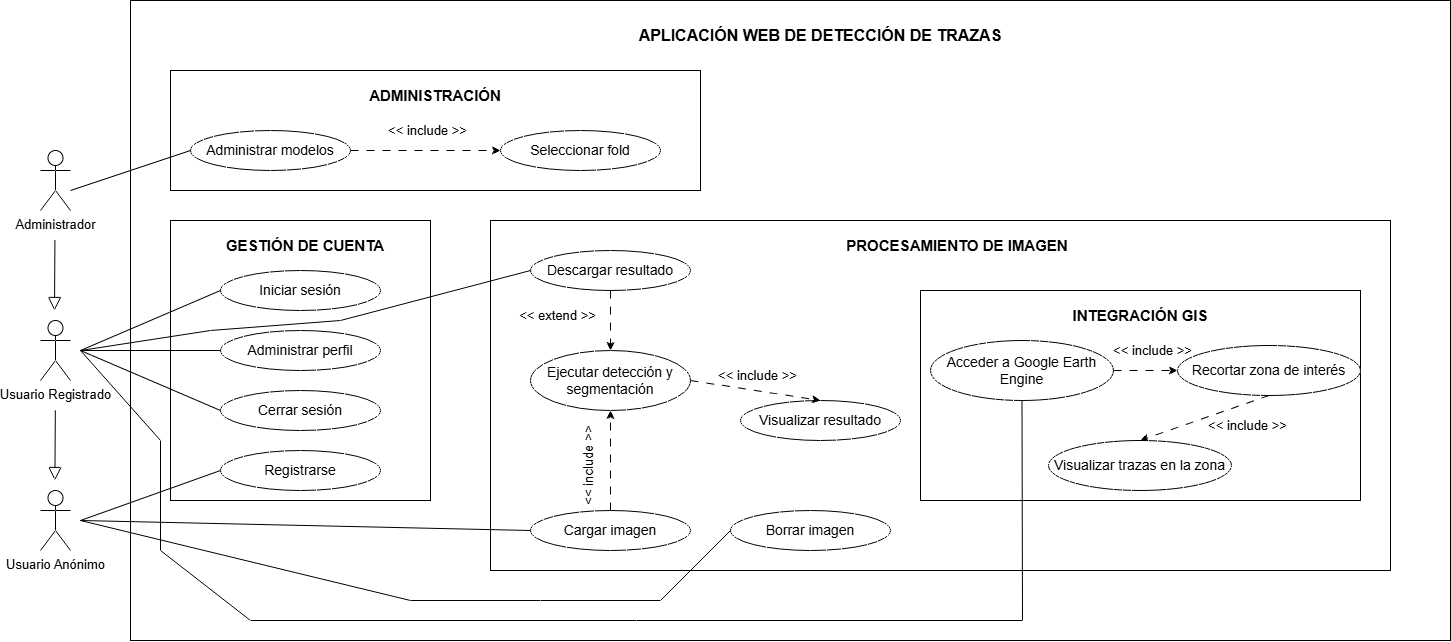
\includegraphics[width=1\linewidth]{img/CasosDeUso}
	\caption[Diagrama de casos de uso de la aplicación]{}
	\label{fig:casosdeuso}
\end{figure}

\subsubsection{Explicación de los casos de uso}

\begin{table}[H]
	\centering
	\footnotesize
	\renewcommand{\arraystretch}{1.2}
	\begin{tabular}{p{3.5cm} p{11cm}}
		\toprule
		\textbf{CU-01 Cargar imagen} & \\
		\midrule
		Actores & Usuario anónimo, Usuario registrado, Administrador \\
		Descripción & Permite al usuario cargar una imagen aérea que será utilizada como entrada para el proceso de detección y segmentación de trazas. \\
		Precondición & El usuario ha accedido a la interfaz de procesamiento. \\
		Flujo principal &
		1) El usuario selecciona una imagen desde su dispositivo.\\
		2) El sistema valida el formato y tamaño del archivo.\\
		3) La imagen queda cargada y disponible para su procesamiento. \\
		Postcondición & Imagen cargada correctamente en el sistema. \\
		Relaciones & Incluido por CU-02 Ejecutar detección y segmentación. \\
		Importancia & Alta \\
		\bottomrule
	\end{tabular}
\end{table}

\begin{table}[H]
	\centering
	\footnotesize
	\renewcommand{\arraystretch}{1.2}
	\begin{tabular}{p{3.5cm} p{11cm}}
		\toprule
		\textbf{CU-02 Ejecutar detección y segmentación} & \\
		\midrule
		Actores & Usuario anónimo, Usuario registrado, Administrador \\
		Descripción & Ejecuta el modelo de detección y segmentación de trazas sobre la imagen cargada. \\
		Precondición & Existe una imagen cargada (CU-01). \\
		Flujo principal &
		1) El usuario inicia el proceso de análisis.\\
		2) El sistema aplica el modelo de detección configurado.\\
		3) Se generan los resultados de segmentación. \\
		Postcondición & Resultado de detección disponible para su visualización. \\
		Relaciones &
		Incluye CU-01 Cargar imagen.\\
		Es incluido por CU-03 Visualizar resultado.\\
		Es extendido por CU-04 Descargar resultado. \\
		Importancia & Alta \\
		\bottomrule
	\end{tabular}
\end{table}

\begin{table}[H]
	\centering
	\footnotesize
	\renewcommand{\arraystretch}{1.2}
	\begin{tabular}{p{3.5cm} p{11cm}}
		\toprule
		\textbf{CU-03 Visualizar resultado} & \\
		\midrule
		Actores & Usuario anónimo, Usuario registrado, Administrador \\
		Descripción & Permite visualizar el resultado de la detección y segmentación superpuesto sobre la imagen original. \\
		Precondición & El proceso de detección se ha ejecutado correctamente (CU-02). \\
		Flujo principal &
		1) El sistema renderiza la imagen original.\\
		2) El sistema superpone el resultado de segmentación.\\
		3) El usuario inspecciona visualmente el resultado. \\
		Postcondición & Resultado visualizado en pantalla. \\
		Relaciones & Incluye CU-02 Ejecutar detección y segmentación. \\
		Importancia & Alta \\
		\bottomrule
	\end{tabular}
\end{table}

\begin{table}[H]
	\centering
	\footnotesize
	\renewcommand{\arraystretch}{1.2}
	\begin{tabular}{p{3.5cm} p{11cm}}
		\toprule
		\textbf{CU-04 Descargar resultado} & \\
		\midrule
		Actores & Usuario registrado, Administrador \\
		Descripción & Permite descargar el resultado de la detección y segmentación para su uso externo. \\
		Precondición & El resultado ha sido generado y visualizado (CU-03). \\
		Flujo principal &
		1) El usuario solicita la descarga del resultado.\\
		2) El sistema genera el archivo correspondiente.\\
		3) El archivo es descargado por el usuario. \\
		Postcondición & Resultado almacenado localmente por el usuario. \\
		Relaciones & Extiende CU-02 Ejecutar detección y segmentación. \\
		Importancia & Media-Alta \\
		\bottomrule
	\end{tabular}
\end{table}

\begin{table}[H]
	\centering
	\footnotesize
	\renewcommand{\arraystretch}{1.2}
	\begin{tabular}{p{3.5cm} p{11cm}}
		\toprule
		\textbf{CU-05 Borrar imagen} & \\
		\midrule
		Actores & Usuario anónimo, Usuario registrado, Administrador \\
		Descripción & Permite eliminar la imagen cargada y reiniciar el flujo de procesamiento. \\
		Precondición & Existe una imagen cargada o un resultado generado. \\
		Flujo principal &
		1) El usuario solicita borrar la imagen.\\
		2) El sistema elimina la imagen y resultados asociados.\\
		3) El sistema vuelve al estado inicial. \\
		Postcondición & Sistema preparado para una nueva ejecución. \\
		Importancia & Media \\
		\bottomrule
	\end{tabular}
\end{table}

\begin{table}[H]
	\centering
	\footnotesize
	\renewcommand{\arraystretch}{1.2}
	\begin{tabular}{p{3.5cm} p{11cm}}
		\toprule
		\textbf{CU-06 Acceder a Google Earth Engine} & \\
		\midrule
		Actores & Usuario registrado \\
		Descripción & Permite acceder al módulo de integración con Google Earth Engine para trabajar sobre una zona geográfica. \\
		Precondición & El usuario ha iniciado sesión. \\
		Flujo principal &
		1) El usuario accede al módulo GIS.\\
		2) El sistema establece conexión con Google Earth Engine.\\
		3) Se habilitan las funcionalidades de recorte y visualización. \\
		Postcondición & Sesión GIS activa. \\
		Relaciones & Incluye CU-06.1 y CU-06.2. \\
		Importancia & Media-Alta \\
		\bottomrule
	\end{tabular}
\end{table}

\begin{table}[H]
	\centering
	\footnotesize
	\renewcommand{\arraystretch}{1.2}
	\begin{tabular}{p{3.5cm} p{11cm}}
		\toprule
		\textbf{CU-06.1 Recortar zona de interés} & \\
		\midrule
		Actores & Usuario registrado \\
		Descripción & Permite definir una zona geográfica de interés mediante un recorte sobre el visor. \\
		Precondición & Acceso al módulo GEE (CU-06). \\
		Flujo principal &
		1) El usuario define el área de recorte.\\
		2) El sistema valida la geometría.\\
		3) La zona queda establecida como área activa. \\
		Postcondición & Zona de interés definida. \\
		Importancia & Media \\
		\bottomrule
	\end{tabular}
\end{table}

\begin{table}[H]
	\centering
	\footnotesize
	\renewcommand{\arraystretch}{1.2}
	\begin{tabular}{p{3.5cm} p{11cm}}
		\toprule
		\textbf{CU-06.2 Visualizar trazas en la zona} & \\
		\midrule
		Actores & Usuario registrado \\
		Descripción & Permite visualizar las trazas detectadas dentro de la zona de interés seleccionada. \\
		Precondición & Zona de interés definida (CU-06.1). \\
		Flujo principal &
		1) El sistema consulta las trazas dentro de la zona.\\
		2) El sistema renderiza las trazas sobre el visor.\\
		3) El usuario inspecciona el resultado. \\
		Postcondición & Trazas visualizadas en la zona seleccionada. \\
		Importancia & Media-Alta \\
		\bottomrule
	\end{tabular}
\end{table}


